\documentclass[10pt,twocolumn]{article}
\usepackage[T1]{fontenc}
\usepackage{lmodern}
\usepackage[letterpaper,margin=0.75in,columnsep=0.3in]{geometry}
\usepackage{microtype}
\usepackage{xcolor}
\usepackage{graphicx}
\usepackage{booktabs}
\usepackage{tabularx}
\usepackage{multicol}
\usepackage{amsmath,amssymb}
\usepackage{algorithm}
\usepackage[noend]{algpseudocode}
\usepackage{tikz}
\usetikzlibrary{arrows.meta,positioning,fit,calc,shapes.geometric}
\usepackage{enumitem}
\usepackage{caption}
\usepackage{xspace}
\usepackage[numbers,sort]{natbib}
\usepackage[colorlinks=true,linkcolor=black,citecolor=blue!50!black,urlcolor=blue!50!black]{hyperref}
\usepackage[capitalise,nameinlink]{cleveref}
\setlist{itemsep=1pt,topsep=3pt}
\captionsetup{font=small,labelfont=bf}
% Placeholders. Every number not yet measured is a \RESULT{key}: a red box reading
% "TBD: run bench". Keys are collected and listed in the TBD appendix. Build with
% \camerareadytrue (see main.tex) and any remaining \RESULT stops the build.
\newif\ifcameraready
\camerareadyfalse
\makeatletter
\newcounter{tbdcount}
\gdef\tbd@list{}
% Measured values live in results-values.tex, generated by eval/fill_v0.py from results.json.
% A key with a value prints it; a key without one stays a red TBD box.
\newcommand{\resdef}[2]{\expandafter\gdef\csname res@#1\endcsname{#2}}
\newcommand{\NM}{\textit{n.m.}}% not measured; each table or paragraph says why
\DeclareRobustCommand{\RESULT}[1]{%
  \ifcsname res@#1\endcsname\csname res@#1\endcsname\else\RESULTTBD{#1}\fi}
\DeclareRobustCommand{\RESULTTBD}[1]{%
  \ifcameraready
    \PackageError{macros}{Unfilled result #1}{Run the benchmark and replace this placeholder with a logged number.}%
  \fi
  \stepcounter{tbdcount}%
  \g@addto@macro\tbd@list{\item\texttt{#1}}%
  \fcolorbox{red!70!black}{red!8}{\textcolor{red!70!black}{\scriptsize\sffamily TBD: run bench}}%
}
\DeclareRobustCommand{\TODO}[1]{%
  \fcolorbox{orange!80!black}{orange!10}{\parbox{0.95\linewidth}{\small\sffamily\textcolor{orange!60!black}{TODO (Rex):} #1}}%
}
\DeclareRobustCommand{\RESULTFIG}[2]{% key, what the figure will show
  \IfFileExists{figures/#1.pdf}{\includegraphics[width=\linewidth]{figures/#1.pdf}}{\RESULTFIGTBD{#1}{#2}}}
\DeclareRobustCommand{\RESULTFIGTBD}[2]{%
  \ifcameraready\PackageError{macros}{Unfilled figure #1}{Draw it with eval/plots.py.}\fi
  \stepcounter{tbdcount}%
  \g@addto@macro\tbd@list{\item\texttt{#1} (figure)}%
  \fcolorbox{red!70!black}{red!5}{\parbox[c][3.2cm][c]{0.9\linewidth}{\centering\sffamily\small
    \textcolor{red!70!black}{TBD: run bench}\\[4pt]\footnotesize #2\\[2pt]\texttt{eval/plots.py} draws this from logged runs.}}%
}
\newcommand{\printtbd}{%
  \ifnum\value{tbdcount}=0 No placeholders remain.\else
  \begin{multicols}{2}\scriptsize\raggedright\begin{itemize}\setlength\itemsep{0pt}\tbd@list\end{itemize}\end{multicols}\fi}
\makeatother
\InputIfFileExists{results-values.tex}{}{}
\InputIfFileExists{results-values-v02.tex}{}{}
\newcommand{\paperversion}{0.1.1}% bumped by scripts/release.sh; 0.1.1 is a paper-only revision (related work and citations)
\newcommand{\codeversion}{0.1.0}% code and benchmark release the results come from
\newcommand{\CR}{Curiosity Recursion\xspace}
\newcommand{\bench}{DarkKin-Bench\xspace}
\newcommand{\pilot}{\textsc{pilot}\xspace}

% \camerareadytrue  % uncomment for camera ready: the build fails while any \RESULT remains

\title{Curiosity Recursion: Durable, Grounded Question Graphs\\for Genealogical Dark Data}
\author{Rex St.\ John\\Lineage / independent researcher\\\texttt{rex@verafy.ai}}
\date{Paper version \paperversion, 26 November 2026. Code, benchmark and data: \url{https://github.com/Verafyai/curiosity-recursion} (v0.1 results from code release v\codeversion; the v0.2 results in \cref{sec:swarm} come from branch \texttt{cr-v0.2}, commit \RESULT{v02-commit}, which is not yet a code release).}

\begin{document}
\twocolumn[\maketitle\vspace{-1em}\begin{center}\begin{minipage}{0.86\textwidth}\small\textbf{Abstract.} Research agents stop early. A person who used an AI assistant to research 65 of his own relatives found that the real work was supervision: typing ``go deeper'', ``are you sure?'', ``did you check the churches?'' and ``did that archive ever reply?'' again and again. Genealogical records make this worse, because many of them are dark data: scanned but unindexed, held by small archives that answer letters weeks later, behind logins, or kept in family boxes. We present \emph{\CR} (CR), a procedure that turns the human nudging loop into an explicit question graph. Every new question must be grounded in a quoted finding, is deduplicated against a persisted memory of every question asked before, and is expanded under breadth, depth, node, budget and time limits with explicit stopping rules. We run CR as a durable workflow on Temporal, so a run survives worker crashes, retries flaky archives, waits days on durable timers, and pauses for a human to approve or redirect it, with the full event history as an audit trail. We also define \emph{\bench}, a benchmark of hidden records about deceased people, stratified by darkness tier, with fault injection and adjudicated scoring; version 0 has 39 subjects and 671 hidden records. A pilot shows the loop surviving repeated worker kills without repeating finished lookups, and an error analysis shows how a quoted-evidence conflict check caught a wrong-parents lead. We report two evaluations, both measured. On the preregistered record-level comparison (\RESULT{n-subjects-test} test subjects, 100 tool calls each), CR found \RESULT{H1-recall-B5-B100} of the hidden records, against \RESULT{H1-recall-B1-B100} for a ReAct agent and \RESULT{H1-recall-B0-B100} for single-pass search: the main hypothesis is not supported. On a corpus-replication benchmark that asks each strategy to rebuild six hand-built family dossiers from a name and birth year alone, with the author's own sites blocked, CR recovered \RESULT{corpus-overall-B5} against \RESULT{corpus-overall-B1} for ReAct and \RESULT{corpus-overall-B0} for single pass, with the highest precision of any strategy (\RESULT{corpus-prec-B5}); a post hoc repair of its question rules reached \RESULT{corpus-overall-B5fix}. None of these differences is significant with six people. The tools could reach only part of each dossier, none of one veteran's facts, and that ceiling limited every strategy more than the choice of strategy did. A preregistered v0.2 (\cref{sec:swarm}) runs parallel lanes as Temporal child workflows behind a shared search ledger that refuses repeat calls; it cut exact repeats to \RESULT{v02-waste-repeat} and used \RESULT{v02-waste-used} of the budget at zero model spend, and its precision (\RESULT{v02-prec-B6-swarm}) was above both comparators, but it recovered \RESULT{v02-overall-B6-swarm} against \RESULT{v02-overall-B1} for ReAct and \RESULT{v02-overall-B5-fix} for the best v0.1 rules: the main v0.2 hypothesis is not supported. Durability held: under injected faults and worker kills both the durable and the plain loop finished every run, but only the plain loop lost and redid finished work. Paper version \paperversion. Code, data and benchmark: \url{https://github.com/Verafyai/curiosity-recursion}.
\end{minipage}\end{center}
\vspace{1em}]
\section{Introduction}
\label{sec:intro}

Anyone who has used a language-model agent for a long research task knows the moment. The agent returns a tidy answer, the answer is incomplete, and the user types ``keep going''. Then ``are you sure that is the same man?'', then ``what about the ship he sailed on?'', then ``did you ever get a reply from the state library?''. The author researched 65 of his own relatives this way with Claude. The agent found real records, but only because a person kept supervising it. By the end, the definition of a thorough search lived in the supervisor's head and in his messages, not in the system. Coming back later with relative 66, there was no way to know whether the agent would check what it had checked for relative 12. A redacted excerpt and counts of those messages by type are not in this version, because the transcripts have not been exported and coded (H5, \cref{sec:results}).

Genealogy makes the problem sharper than most research, for two reasons. First, the records are dark data in the sense of \citet{heidorn2008dark} and \citet{hand2020dark}: they exist, but the systems that should find them cannot see them. A regimental history names a soldier on page 14 of a scanned book with no name index. A town clerk holds a marriage register and answers by mail. A church register, a ship's crew list, or a box of letters in a cousin's closet may be the only source. Second, the work is long. A letter to an archive can take three weeks to answer, and following up on it is part of the research. A chat window cannot wait three weeks, and a script that crashes on day four loses its place.

This paper turns the supervisor's loop into a system and proposes a way to measure it. Our claim is falsifiable: \emph{at equal tool-call budget, a durable \CR agent finds more verifiable hidden records of deceased people than single-pass, ReAct and checklist-only agents, without lowering claim precision.} We built the system and the benchmark, preregistered the comparison (\cref{sec:bench}), and ran it. The claim is not supported: at 100 tool calls a ReAct agent found more than the preregistered CR on both evaluations, and CR's advantages were precision and durability, not recall (\cref{sec:corpus,sec:results}).

\paragraph{Contributions.}
\begin{enumerate}
\item \textbf{\CR (CR)}, a procedure that turns the human ``keep digging'' loop into an explicit question graph. Each new question must be grounded in a specific prior finding, is deduplicated against a persisted question memory, is scored for novelty and expected yield, and is expanded under breadth, depth, node and time budgets with explicit stopping rules (\cref{sec:loop}).
\item \textbf{\bench}, a benchmark for long-horizon archival research on deceased people, with hidden ground-truth records stratified by darkness tier, an adjudication protocol, cost accounting, and fault injection: worker kills, flaky archives, multi-day waits and delayed archive replies (\cref{sec:bench}).
\item \textbf{A durable, auditable reference system}: CR plus heritage circuits, run on Temporal (retries, durable timers, signals for human approval and redirection, full event history), with evidence discipline (claim tiers, every published sentence tied to claim ids). It is released as open code, and the paper reports where durability and memory matter and where they do not (\cref{sec:solution,sec:results}).
\end{enumerate}

\noindent We are careful about what we do not claim. A name found in OCR text is a lead, not an identification. In the pilot, most record-level facts come from curated evaluation fixtures, labelled as stubs; live sources add leads. The generator in the current system is rule-based. All of this is stated where it applies and collected in \cref{sec:limits}.

\section{Related work}
\label{sec:related}

\paragraph{Reasoning and acting agents.} ReAct interleaves reasoning traces and tool actions on one trajectory \citep{yao2023react}. Reflexion adds verbal self-feedback across attempts \citep{shinn2023reflexion}, and Self-Refine iterates on its own output \citep{madaan2023selfrefine}. Tree of Thoughts searches over intermediate reasoning states with a model as evaluator \citep{yao2023tot}. Self-Ask decomposes a question into follow-up sub-questions answered in turn \citep{press2023selfask}, and IRCoT interleaves retrieval with chain-of-thought steps \citep{trivedi2023ircot}. Toolformer teaches a model when to call tools \citep{schick2023toolformer}. Voyager keeps an automatic curriculum and a growing skill library, a form of persisted exploration \citep{wang2023voyager}. \Cref{sec:loop} contrasts CR with these methods.

\paragraph{Deep research and web agents.} WebGPT answers questions by browsing with human feedback \citep{nakano2021webgpt}. STORM writes Wikipedia-like articles after generating questions from several simulated perspectives \citep{shao2024storm}, the closest prior use of question generation to drive coverage. Commercial \citep{openai2025deepresearch} and open-source \citep{elovic2023gptresearcher} deep-research agents run multi-step research in one session; none is built to wait weeks for a letter, survive a crash, or prove which sources it checked.

\paragraph{Agent benchmarks.} WebArena \citep{zhou2024webarena}, GAIA \citep{mialon2024gaia}, BrowseComp \citep{wei2025browsecomp}, SWE-bench \citep{jimenez2024swebench} and DeepResearch Bench \citep{du2025deepresearchbench} measure agents on web tasks, hard-to-find facts, code and research reports. To our knowledge, none scores hidden archival records by how dark they are, counts a correctly drafted request to an offline archive as a find, or injects crashes and multi-day waits.

\paragraph{Curiosity, novelty and active questioning.} Intrinsic-motivation work rewards an agent for what it cannot yet predict \citep{pathak2017curiosity,schmidhuber2010creativity}. Novelty search abandons the objective and rewards behaviour that differs from what came before \citep{lehman2011novelty}. Active learning chooses the queries whose answers are most informative \citep{settles2009active}, and neural question generation learns to ask questions about a text \citep{du2017learning}. CR borrows the reward for novelty, but applies it to a space of questions whose payoff is external and checkable: a record exists or it does not.

\paragraph{Record linkage and genealogy data.} Probabilistic record linkage \citep{fellegi1969linkage} and its large-scale historical uses \citep{abramitzky2021linking,price2021censustree} decide when two records describe one person. CR treats a name match as a lead and leaves identity to evidence and review (\cref{sec:wrongparents}).

\paragraph{Archives and dark data.} Dark data and handwriting recognition are discussed in \cref{sec:darkdata}; the FAIR principles describe what findable data needs \citep{wilkinson2016fair}, and we document the benchmark with a datasheet \citep{gebru2021datasheets}.

\paragraph{Durable execution.} Sagas split a long-lived transaction into steps with compensations \citep{garciamolina1987sagas}. Durable Functions give stateful serverless code replay semantics \citep{burckhardt2021durable}. Temporal records every workflow step in an event history and replays deterministic workflow code to recover state \citep{temporaldocs,temporalpythonsdk}. We use it because the research loop is a long-lived process with external side effects, timers measured in weeks, and a human in the loop.

\section{Problem}
\label{sec:problem}

\paragraph{Task.} Long-running, deep, agentic genealogical research on one deceased person: find records about them, deepen each lead, broaden to new kinds of sources, brainstorm and iterate, send and follow up direct research requests to archives over weeks, and ingest what comes back so that it can become a cited chapter or newsletter.

\paragraph{Input.} A subject card: a name and variant spellings, birth and death years with their precision (exact, about, before, after), places, optional family notes, and an optional research question. \paragraph{Output.} A question graph with every question, why it was asked and what came back; documented claims, each with a source; leads, labelled as leads with their quoted text; named conflicts; drafted research requests awaiting approval; and a report written only from documented claims.

\paragraph{Constraints.} (1) Deceased people only: a living-person gate runs before any lookup (\cref{sec:gate}). (2) Cite everything: every published sentence carries claim ids. (3) Ask before outreach: nothing is sent; an approved request is written to a file. (4) No scraping where terms forbid it, and no captcha or paywall bypass. (5) A name match is never an identification, and a surname alone never links two people.

\subsection{Failure modes of plain agents}
\label{sec:failures}

These came from the 65-relative work. Redacted transcript examples are not included in this version.
\begin{description}[leftmargin=1.2em,labelindent=0pt,font=\normalfont\bfseries]
\item[F1] No follow-up on direct queries to small archives: nothing is sent, or a pending reply is forgotten.
\item[F2] No download, index, ingest or archive of what it receives: the answer lives in a chat scroll, not a record store.
\item[F3] Stops being curious: does not chase the new leads a finding opens.
\item[F4] Does not brainstorm from its current record: new facts do not produce new questions.
\item[F5] Needs constant reminders to keep going.
\item[F6] Does not think of new sources: churches, synagogues, ship crew lists, school registers, regimental histories.
\item[F7] Becomes a black box: no record of what it checked, so thoroughness can be neither trusted nor repeated.
\item[F8] Loses state on a crash, a timeout or a context limit, and cannot wait days.
\end{description}

\section{Genealogical dark data}
\label{sec:darkdata}

We use \emph{dark data} for records that exist but are not visible to the systems that should find them \citep{heidorn2008dark,hand2020dark}. Genealogical records are dark in several ways at once. They are fragmented across many small holders: historical societies, town clerks, churches and synagogues, museums and veterans' archives. Many are digitised without an index, as page images or OCR text in scanned books and newspapers, so a catalogue name search misses them while full-text search, or handwriting recognition such as Transkribus \citep{kahle2017transkribus}, can find them. Some have no finding aid and can be reached only by a manual lookup or a letter. Families hold boxes of slides, photographs, books, letters and clippings. Other records sit behind logins, paywalls or captchas. All are noisy: variant spellings, transcription errors, two people with one name \citep{fellegi1969linkage,abramitzky2021linking,price2021censustree}; some are destroyed, so an absence must be recorded as an absence. Most important for this paper, many are found only by asking the right next question, and by following up on replies that arrive weeks later.

\begin{center}

\fbox{\parbox{0.93\linewidth}{\small
\textbf{Darkness tiers} (per record).\quad
\textbf{T0, online indexed:} reachable by a structured search or API (a catalogue record, an index entry, a Wikidata statement).\quad
\textbf{T1, online full text only:} online only as OCR text or page images (digitised books, newspapers); finding it needs full-text search and page location.\quad
\textbf{T2, online gated:} behind a login, OAuth, a paywall or a captcha. Scored as identification: the right holding is named and a correct request is drafted. Never fetched by bypass.\quad
\textbf{T3, offline only:} an archive, church, synagogue, town clerk, museum or family box. Scored as identification plus a correct outreach draft: right holder, right record, right identifiers.}}
\end{center}

\section{Analysis: what the human supervisor was doing}
\label{sec:analysis}

Read back, the nudges are not random. The supervisor was running a loop with four parts: \emph{memory} (what has been asked, what is pending, which archive has not replied), \emph{judgement about what is missing} (there is a unit, so where are the regimental books?), \emph{scepticism} (is this the same man?), and \emph{patience} (wait for the letter, then follow up). A chat window loses the memory when the context fills, cannot wait, leaves no record of what it checked, and has no notion of ``asked before''. A plain script has the memory only until it crashes. \Cref{tab:fmm} maps each failure mode to the mechanism that addresses it and the metric that tests it.

\begin{table*}[t]
\centering\small
\begin{tabularx}{\textwidth}{@{}l>{\raggedright\arraybackslash}X>{\raggedright\arraybackslash}X@{}}
\toprule
Failure mode & Mechanism & Metric \\
\midrule
F1 no follow-up on small archives & Outreach drafts as workflow state, durable timers, reply signals & Follow-up completion; T3 identification recall \\
F2 no ingest or archive & Every finding persisted per level; citations with item ids and page & Records persisted / found; page-located citations \\
F3 not curious on new leads & Recursive expansion conditioned on each node's finding & Lead-chain depth to hit; recall at depth $\ge 2$ \\
F4 no brainstorm from record & Grounded generator over the evidence state $R$ & Share of hits found by question nodes vs.\ checklist \\
F5 needs reminders & Loop runs to a stopping rule, not to a reply & Nudge coverage; human interventions per run \\
F6 no new sources & ``Where else?'' nodes; tier bonus & Novel-source discovery rate \\
F7 black box & Question graph, event history, checklist coverage & Coverage report completeness; replay success \\
F8 lost state, cannot wait & Temporal workflow & Completion under faults; duplicate-work ratio \\
\bottomrule
\end{tabularx}
\caption{Failure modes, the mechanism in the system for each, and the metric in \bench that tests it.}
\label{tab:fmm}
\end{table*}

\section{The research loop: \CR}
\label{sec:loop}

\subsection{Objects}
A \emph{subject} $s$ is a deceased person with name variants, birth and death years with precision, places, family notes and a research question. The \emph{evidence state} $R_t$ is the set of findings so far. A finding has a source, a mode (\emph{live}, from a public endpoint, or \emph{stub}, from a curated fixture or a source that needs a human), a status, claims (each with a tier: documented, told, lore or inferred) and citations (URL, title, item id, snippet, and a name-match strength). The \emph{question graph} $G=(V,E)$ has one node per question. A node $v$ carries its text $q_v$, its parent $p(v)$, the finding that sparked it $f_v$ (the ``because'', quoted), a plan $\pi_v=(\text{handler},\text{query})$, a status in \{pending, running, answered, no\_lead, stub, error, skipped\}, its answer, citations, snippets, attempts and failures, its depth $d(v)$ and its round. $E$ holds the edges $(p(v),v)$. The root is $s$; level 0 is the circuit checklist. The \emph{question memory} $M$ holds every question ever asked for this subject key (and, for H3, similar subjects), keyed by a canonical key $\kappa(q)$. The budgets are the breadth $b$ (questions picked per expanded node), the depth limit $d_{\max}$, the node budget $N$, the tool-call budget $B$, the wall-clock budget $T$, and the pause between levels $\tau$, a durable timer.

\subsection{Generate, dedupe, score, select}
\paragraph{Generator.} $g(s,R,v,M)$ returns candidate questions $C$. \emph{Grounding constraint:} every $c\in C$ must name a finding $f_c\in R$, or the node or checklist gap that sparked it, and quote it. A candidate with no spark is rejected and counted. This is the difference from free brainstorming: curiosity is anchored to evidence, so the graph is auditable. The rule-based generator (the one measured in the pilot) has lead templates keyed on what a finding contains: a military unit leads to regimental books and newspapers; a ship to voyages and crew lists; a ``son of A and B'' line to the parents; a marriage, school or congregation to its registers; a death year to an obituary; a book hit to a search inside that book for the page. A grounded model generator is implemented behind the same activity and must return a spark id and a quote that the code checks against the spark text; it has not been measured.

\paragraph{Dedupe.} Drop $c$ if $\kappa(c)\in M$ or $\kappa(c)$ is already in $V$. $\kappa$ is a normalised template key, for example \texttt{unit-books:12th-connecticut-infantry}. For model-written questions, which reword freely, a near-duplicate test also drops $c$ when its similarity to any asked question is at least $\theta$; we use the larger of word-set Jaccard and a character-sequence ratio, with $\theta=0.85$.

\paragraph{Score.} In general,
\begin{multline}
\mathrm{score}(c)=w_y\,\mathrm{yield}(\mathrm{tmpl}(c))+w_n\,\mathrm{novelty}(c)\\
+w_r\,\mathrm{rel}(c,\text{question})+w_t\,\mathrm{tier}(c)-w_c\,\mathrm{cost}(c),
\end{multline}
with $\mathrm{novelty}(c)=1-\max_{a\in M\cup V}\mathrm{sim}(c,a)$. The current implementation uses fixed integer template scores plus 2 when the user's research question mentions the topic; the weighted form is the general case that the ablations vary.

\paragraph{Select.} Pick the top $b$ live candidates, plus up to 2 stub candidates (questions that need a human or a letter, such as a pension file at the National Archives), and hold back up to 12 as ``not yet asked'', shown in the dashboard.

\subsection{Expand, nudge, stop}
\paragraph{Expansion is the recursion.} For each picked node, investigate it (an activity with retries), add its finding to $R$, and call $g$ again \emph{conditioned on that node's own finding}. That conditioning gives lead chains: ``book found'' leads to ``does that book name him, and on which page?'', which leads to ``are you sure it is the same Erastus?''.

\paragraph{Built-in nudges.} An answered node whose match is weak (surname only, or a newspaper hit without place) spawns an ``Are you sure?'' verification question. Every node spawns a ``Where else might this be?'' question that switches source family, books to newspapers or back. A checklist gap spawns ``Still nothing on $X$: where else could it be?''. A person can inject a question at any time with a signal (``Dig here first''); it joins the next level and is followed to the same depth.

\paragraph{Stopping rules.} Each run records which rule fired: (1) the frontier is empty, no new grounded, non-duplicate question; (2) $|V|$ reaches $N$; (3) the tool-call count reaches $B$; (4) elapsed time reaches $T$; (5) depth reaches $d_{\max}$. Proposed but not implemented: (6) marginal yield, new verified records per node, below $\epsilon$ for $k$ consecutive levels.

\begin{algorithm*}[t]
\caption{\CR as a durable workflow. Lines marked $\triangleright$ are activities: recorded in event history, retried, never repeated after they finish.}
\label{alg:cr}
\footnotesize
\begin{algorithmic}[1]
\Procedure{CuriosityRecursion}{$s$, circuits, $b$, $d_{\max}$, $N$, $B$, $T$, $\tau$, $M$}
\State \textsc{Gate}$(s)$ \Comment{living-person gate, deterministic, in workflow code}
\State $R \gets$ \textsc{RunChecklist}(circuits$(s)$) $\triangleright$ \Comment{level 0, parallel, each step retried}
\State $F \gets$ \textsc{Reask}$(M, s, \text{limit}=b)$ \Comment{memory: recheck earlier top-level questions first}
\State $F \gets F \cup \textsc{Select}(\textsc{Dedupe}(g(s,R,\text{root},M),M),b)$ $\triangleright$
\While{$F \neq \emptyset$}
  \State $\mathit{next} \gets [\,]$
  \ForAll{$v \in F$ \textbf{in parallel}}
    \State $v.\mathit{finding} \gets$ \textsc{Investigate}$(v)$ $\triangleright$ \Comment{retry with backoff}
    \State $R \gets R \cup \{v.\mathit{finding}\}$
    \If{$d(v) < d_{\max}$} $\mathit{next} \gets \mathit{next} \cup \textsc{Select}(\textsc{Dedupe}(g(s,R,v,M),M),b)$ $\triangleright$ \EndIf
  \EndFor
  \State \textsc{Persist}$(V, M)$ $\triangleright$ \Comment{every level, every question}
  \If{$\mathit{next}=\emptyset$ \textbf{or} $|V|\ge N$ \textbf{or} calls $\ge B$ \textbf{or} time $\ge T$} \textbf{break} \EndIf
  \State \textsc{DurableSleep}$(\tau)$ \Comment{survives restarts; minutes to weeks}
  \State $F \gets \mathit{next} \cup \textsc{HumanRedirects}()$
\EndWhile
\State $\mathit{report} \gets$ \textsc{Compose}$(R)$ $\triangleright$ \Comment{only documented claims become prose; leads quoted as leads}
\State wait for an \textsc{Approve} or \textsc{Reject} signal, with timeout; \textsc{Redirect} signals reopen the loop
\State \Return $\mathit{report}, G$
\EndProcedure
\end{algorithmic}
\end{algorithm*}

\subsection{Worked example}
\label{sec:worked}
\Cref{fig:graph} is a real run for Erastus W.\ Burnham (1834 to 1921) on the Civil War veteran circuit (run \texttt{studio-erastus-w-burnham-1126-110934}, 25 nodes). Level 0 ran 16 checklist steps; its unit facts came from a curated fixture and are labelled stub. Memory re-asked three top-level questions from earlier runs. One of them, \textit{r3}, asked ``Which books cover the 12th Connecticut Infantry, and do they name him?'' and found two candidate books on Internet Archive by catalogue title search (live). At level 2, \textit{r3.2} searched inside one of them, \emph{The Twelfth Regiment, Connecticut Volunteer Infantry in the War of the Rebellion}, and found a roster on page image 14 that reads, verbatim, ``Burke, John Burnham, Erastus W.\ Carlan, John''. The roster lists surname first in alphabetical order, so ``Burnham, Erastus W.''\ is an entry. Its first attempts failed with simulated 503 errors and Temporal retried them. This is a T1 find: the roster is online, but in no name index the agent was given. It is a lead, a full-name match, not an identification.

\begin{figure*}[t]
\centering
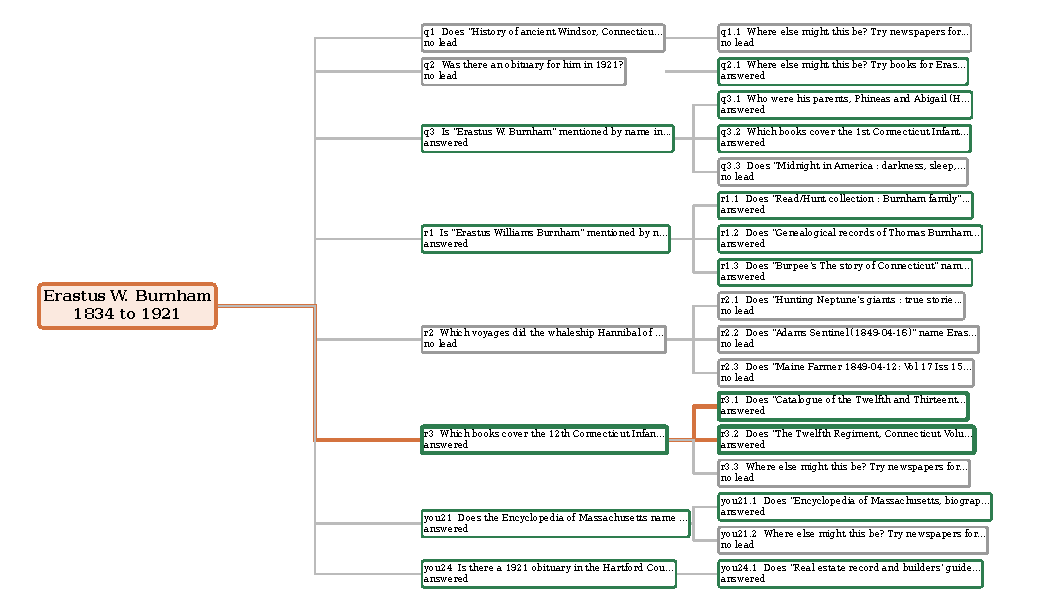
\includegraphics[width=0.92\textwidth,height=0.34\textheight,keepaspectratio]{figures/fig4-graph.pdf}
\caption{A real question graph (Erastus W.\ Burnham, 25 nodes), left to right: the person, then each question with its status written on the node. Highlighted: the 12th Connecticut chain, \textit{r3} (which books cover the regiment?) to \textit{r3.2} (does this book name him, on which page?), which reached the roster on page image 14. Ids \textit{r1} to \textit{r3} were re-asked from memory; \textit{you21} and \textit{you24} were injected by the reviewer.}
\label{fig:graph}
\end{figure*}

\subsection{Relation to prior search methods, and cost}
Tree of Thoughts searches over internal reasoning states with a model evaluator \citep{yao2023tot}; ReAct interleaves thought and action on one trajectory \citep{yao2023react}; Self-Ask decomposes a question into sub-questions \citep{press2023selfask}. CR differs in three ways: its nodes are questions to the outside world whose answers are evidence; generation is grounded in a cited finding; and the question set is persisted and reused across runs and subjects. Novelty search \citep{lehman2011novelty} and curiosity-driven exploration \citep{pathak2017curiosity,schmidhuber2010creativity} motivate rewarding novelty, but CR applies it to a question space with an external, verifiable payoff.

The graph has at most $\min(N,\sum_{k=1}^{d_{\max}} b^k)$ live nodes, plus up to 2 stub children per expanded node. Cost is linear in $|V|$ tool calls plus one generator call per expanded node. Event history also grows linearly in $|V|$: the 25-node run above ended at 303 events and 1.74\,MB of history. Week-long or 500-node runs need Temporal's continue-as-new with $(V,M)$ as compact state, or one child workflow per first-level subtree; neither is implemented yet.

\section{Solution: circuits, durable execution and the system}
\label{sec:solution}

\subsection{Circuits: a floor, not a ceiling}
A \emph{circuit} is a named baseline checklist for a heritage or kin group: Civil War veteran, the crossing (immigration), and a vital-records life story in the reference code, with more in the production system. Each circuit lists topics (unit and service dates, burial, pension file, census households, parents) and, for each topic, the steps that can fill it, in order. A step is \emph{live}, a keyless public client, or a \emph{stub}, a source that needs a login, a key, a letter or a visit, with the reason written next to it. ``Did you check the synagogues?''\ becomes a line item that is checked or not. After level 0 each topic is \emph{covered} (a documented claim), \emph{leads only} (candidate citations) or \emph{missing}; missing topics become grounded ``still nothing on $X$'' questions. Circuits make thoroughness repeatable: relative 66 gets the same floor as relative 12, and the coverage table says so.

\subsection{Durable execution on Temporal}
The loop runs as a Temporal workflow \citep{temporaldocs,temporalpythonsdk}. Workflow code is deterministic: it decides, and every side effect is an \emph{activity} (a catalogue search, a full-text search, a search inside a book, writing to the question store, composing the report). Temporal records each activity's result in the workflow's \emph{event history}; if the worker process dies, a new worker replays the history to rebuild state and continues from the same node without repeating finished lookups. This is the same idea as sagas for long-lived transactions \citep{garciamolina1987sagas} and replay-based durable functions \citep{burckhardt2021durable}. \Cref{fig:loop} shows the loop as it runs. The pieces CR uses:
\emph{Retry policies}: live lookups retry with exponential backoff (2\,s initial, doubling, 30\,s maximum, 8 attempts); a 4xx response, such as Internet Archive refusing inside-book search on a lending-library book (HTTP 403), is recorded as ``source refused'' and not retried. \emph{Durable timers} separate levels, from seconds to weeks. \emph{Signals} carry \texttt{approve}, \texttt{reject}, \texttt{redirect} (``dig here first''), \texttt{outreach\_decision} and \texttt{archive\_reply}, an archive's answer, verbatim. A \emph{query}, \texttt{progress}, returns the typed graph the interface draws. The checklist runs as a \emph{child workflow} with its own history. The \emph{event history} is the audit trail: every question, retry, timer and human decision, replayed against current code by a test in the repository.

\begin{figure}[t]
\centering
\resizebox{\columnwidth}{!}{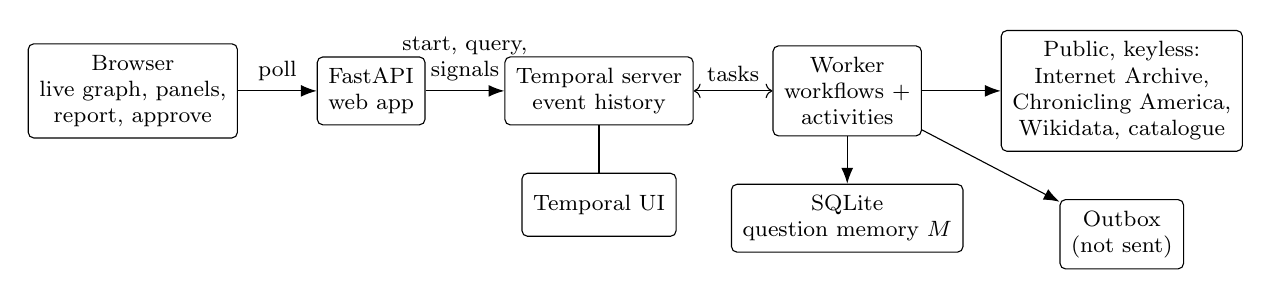
\begin{tikzpicture}[font=\footnotesize, node distance=4mm and 6mm,
  box/.style={draw, rounded corners=2pt, align=center, inner sep=4pt, minimum height=8mm},
  grp/.style={draw, dashed, rounded corners=3pt, inner sep=5pt}, ar/.style={-{Latex[length=2mm]}}]
\node[box] (ui) {Browser\\live graph, panels,\\report, approve};
\node[box, right=10mm of ui] (api) {FastAPI\\web app};
\node[box, right=10mm of api] (t) {Temporal server\\event history};
\node[box, below=6mm of t] (tui) {Temporal UI};
\node[box, right=10mm of t] (w) {Worker\\workflows +\\activities};
\node[box, below=6mm of w] (db) {SQLite\\question memory $M$};
\node[box, right=10mm of w] (src) {Public, keyless:\\Internet Archive,\\Chronicling America,\\Wikidata, catalogue};
\node[box, below=6mm of src] (out) {Outbox\\(not sent)};
\draw[ar] (ui) -- node[above]{poll} (api);
\draw[ar] (api) -- node[above, align=center]{start, query,\\signals} (t);
\draw[ar, <->] (t) -- node[above]{tasks} (w);
\draw (t) -- (tui);
\draw[ar] (w) -- (db); \draw[ar] (w) -- (out); \draw[ar] (w) -- (src);
\end{tikzpicture}}
\caption{System architecture. The web app never runs research itself: it starts workflows, reads the \texttt{progress} query and sends signals. Workers poll Temporal for tasks, call public keyless sources, and write the question memory and approved letters (never sent).}
\label{fig:arch}
\end{figure}

\begin{figure}[t]
\centering
\resizebox{\columnwidth}{!}{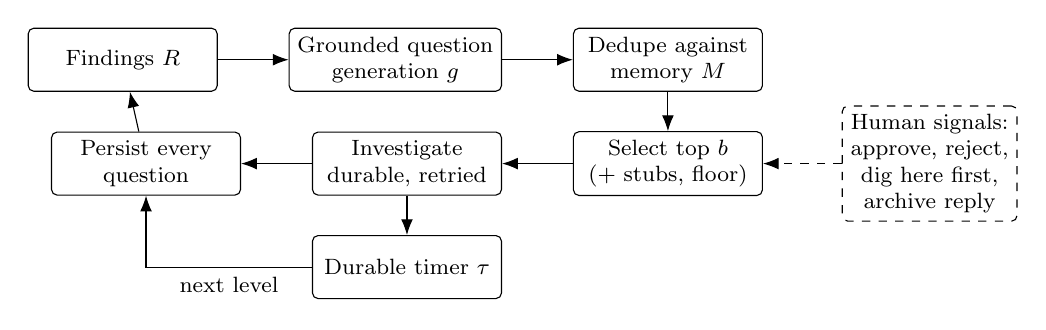
\begin{tikzpicture}[font=\footnotesize, node distance=5mm and 9mm,
  st/.style={draw, rounded corners=2pt, align=center, inner sep=3pt, minimum width=24mm, minimum height=8mm},
  ar/.style={-{Latex[length=2mm]}}, hm/.style={draw, dashed, rounded corners=2pt, align=center, inner sep=3pt}]
\node[st] (find) {Findings $R$};
\node[st, right=of find] (gen) {Grounded question\\generation $g$};
\node[st, right=of gen] (dd) {Dedupe against\\memory $M$};
\node[st, below=of dd] (sel) {Select top $b$\\(+ stubs, floor)};
\node[st, left=of sel] (inv) {Investigate\\durable, retried};
\node[st, left=of inv] (per) {Persist every\\question};
\node[st, below=of inv] (sleep) {Durable timer $\tau$};
\draw[ar] (find) -- (gen); \draw[ar] (gen) -- (dd); \draw[ar] (dd) -- (sel); \draw[ar] (sel) -- (inv);
\draw[ar] (inv) -- (per); \draw[ar] (per) -- (find);
\draw[ar] (inv) -- (sleep); \draw[ar] (sleep.west) -| node[near start, below]{next level} (per.south);
\node[hm, right=10mm of sel] (h) {Human signals:\\approve, reject,\\dig here first,\\archive reply};
\draw[ar, dashed] (h) -- (sel);
\end{tikzpicture}}
\caption{The research loop. Every finding sparks grounded questions; duplicates of anything asked before are dropped; the best $b$ are investigated as durable activities; every question is persisted; a durable timer separates levels. People approve, reject or redirect by signal at any time.}
\label{fig:loop}
\end{figure}

\subsection{The Studio Builder system}
The reference system (\cref{fig:arch}) has typed schemas for every value that crosses Temporal (Pydantic models with Temporal's Pydantic data converter, so the Temporal UI shows real field names), a live graph user interface, and panels for open questions, answered questions, outgoing research requests, failures and retries, checklist coverage and the run log.

\label{sec:gate}\paragraph{Living-person gate.} Before any lookup, deterministic workflow code applies the rule of the production system's gate: research runs only if a death year is on record (and its precision is not ``after''), or the birth year is at least 110 years ago. An unknown date means presumed living, and that default is never flipped.

\paragraph{Outreach is ask first.} A stub question that needs a human (a pension file, a town clerk, a museum collection) becomes a drafted letter that points to where the holder lists its real address and is signed ``[Your name]''. It waits for an \texttt{outreach\_decision} signal. Approving writes a text file; there is no mail transport in the code, and a test checks that.

\paragraph{Evidence discipline.} Claims have tiers: \emph{documented} (a record), \emph{told} (the family says), \emph{lore}, \emph{possible} (a lead: an OCR or search-snippet match, shown with its quote) and \emph{inferred} (reasoning only, never published). The report is written only from documented and told claims; every sentence carries claim ids; a validator drops a sentence that cites a lead, states an interior state, makes a causal link no record makes, tells a family story outside ``Your family remembers that'', or uses a number no cited record holds. Disagreements are named as conflicts and never resolved, and leads from the same passage join the conflict (\cref{sec:wrongparents}).

\section{\bench}
\label{sec:bench}

\subsection{Subjects, records and tiers}
Version 0 is built by a script (\texttt{bench/convert\_kin.py}) from two evaluation sets of the production system. The first holds 4 family dossier subjects built from the author's research (born 1834 to 1921, died 1921 to 2006) with 523 expected records. The second holds 35 public historical figures who died before 1990, 7 each in five groups (Jewish, academic, immigrant, military, control), researched by separate agents from Wikipedia, Wikidata and the archives themselves, not by the code builder, with 148 records. A further 15 public figures are in a holdout file that we have sealed unread; its hash is in the preregistration and it is scored once, at the end. Every subject passed the living-person gate, and the build log records each decision. \Cref{tab:data} gives the counts. Tiers come from a host rule and are marked unconfirmed until a person checks each record. Version 1 adds the author's remaining dossiers and 100 to 200 public figures chosen by a fixed hash, by people who do not tune the system. The remaining family dossiers are used in a separate corpus-replication benchmark (\cref{sec:corpus}); record tiers in v0 are as assigned by the conversion script and were not re-checked by hand.

\begin{table*}[t]
\centering\small
\begin{tabular}{@{}lr@{\qquad}lr@{\qquad}lr@{}}
\toprule
Subjects & 39 & Records (hidden) & 671 & Split dev / test & 27 / 12 \\
Family dossiers & 4 & T0 online indexed & 156 & Born before 1850 & 9 \\
Public figures & 35 & T1 full text only & 467 & Born 1850 to 1899 & 18 \\
Sealed holdout (unread) & 15 & T2 gated & 17 & Born 1900 to 1949 & 12 \\
Removed by living gate & 0 & T3 offline only & 31 & Private items (counts only) & 32 \\
\bottomrule
\end{tabular}
\caption{\bench v0 (from \texttt{bench/data/stats.json}). Tiers are by host rule and not yet confirmed by a person. Family dossiers include some period-context sources that a reviewer will remove from the denominator.}
\label{tab:data}
\end{table*}

\paragraph{Hidden-record protocol.} The subject card holds only seed facts: name, years and places. Every record is hidden and scored; the production system's Wikipedia and Wikidata ids are withheld from the card because they would hand over ground truth. A subject-level test split of 30\%, chosen by a fixed hash, is never looked at while rules, templates, prompts or circuits change. Every agent runs with the evaluation fixtures switched off, since they hold ground truth.

\subsection{Agents at equal budget}
All agents get the same sources, tools, rate limits and budgets. The budget $B$ counts tool calls (checklist steps plus investigations), with tokens, dollars and wall-clock time also logged; $B\in\{25,50,100,200\}$. \textbf{B0} is a single-pass model agent: one search-and-answer pass. \textbf{B1} is ReAct \citep{yao2023react} with the same tools, run until it stops or spends $B$. \textbf{B2} is the human-nudged reference: the author's real transcripts, scored for records reached and nudges per verified record; it is not run at equal budget. \textbf{B3} is checklist-only circuits (level 0). \textbf{B4} is the same CR code in a plain asyncio loop with in-process retries and no persistence. \textbf{B5} is the full system. An optional \textbf{B6} is a commercial deep-research agent \citep{openai2025deepresearch}, only where its terms allow, with the date and cost reported. Configurations that use a model or faults run with 3 seeds.

\subsection{Metrics}
\emph{Hidden-record recall@$B$} is the number of found and verified hidden records over the number of hidden records, overall and by tier (T2 and T3 count identification). We report the \emph{recall-versus-budget curve} and its area. \emph{Claim precision} is verified documented claims over documented claims asserted; \emph{lead precision} is reported separately, since leads may be wrong but must be labelled. The \emph{wrong-person rate} counts claims or records attributed to the subject that belong to someone else, and the \emph{hallucination rate} counts records or citations that do not exist or do not contain the claimed text (target 0 for documented claims). The \emph{novel-source discovery rate} counts distinct hosts or archives holding hidden records that the agent found and that are not in the circuit checklist or seed catalogue. \emph{Lead-chain depth to hit} is the depth of the node that first found each record (checklist hits are depth 0). We also report time to first hit, cost per verified record, completion under faults, the \emph{duplicate-work ratio} (activities re-executed after a crash over activities completed), question diversity and the grounded share (100\% required for CR), human interventions per run, and \emph{nudge coverage}: the share of the human's coded nudges (\cref{tab:nudge}) whose intent the agent generated on its own.

\subsection{Faults, adjudication and statistics}
\paragraph{Fault injection (H2).} Worker kills by SIGKILL at exponential intervals, with a restart after a delay; flaky archives that fail the first $k$ attempts of a lookup with probability $p\in\{0,0.1,0.3,0.5\}$, plus the real permanent refusals; multi-day level pauses and outreach waits of 3 to 21 days run on Temporal's time-skipping test server; and simulated archives that answer a drafted request by signal after a delay, with a record, with ``no record'', or never. Each run records whether it completed, its stop reason, history size, repeated activities and final recall.

\paragraph{Adjudication.} Two independent raters, at least one an experienced genealogist who did not build the system, label every item blind to the agent: correct and same person; correct record, wrong person; real source that does not support the claim; source does not exist; or cannot determine. We require Cohen's kappa \citep{cohen1960kappa} of at least 0.7 before scoring; a third rater resolves disagreements. Model judges may be a secondary rater with their agreement reported, never the only one. Automatic URL and identifier matches are candidates until adjudicated.

\paragraph{Statistics.} Per-subject paired comparisons: Wilcoxon signed-rank for recall and cost, exact McNemar for completion, bootstrap 95\% confidence intervals (10{,}000 resamples) for every headline number, Holm correction across comparisons, and effect sizes. Every table caption states the number of subjects and seeds. The hypotheses, budgets, margins and tests are preregistered (\texttt{bench/PREREGISTRATION.md}).

\paragraph{Hypotheses (preregistered).} \textbf{H1}: at equal $B$, B5 has higher recall@$B$ than B0, B1 and B3; falsified if B5 is not better than B3 at $B\in\{50,100,200\}$; H1b, the gain is largest in T1 and T3 and smallest in T0. \textbf{H2}: under faults, B5 completes more runs and repeats less work than B4; falsified if completion does not differ at $p=0.3$ with kills. \textbf{H3}: with memory on, a repeat or similar-subject run reaches the first run's recall with fewer tool calls; falsified if cost does not fall. \textbf{H4}: B5's documented-claim precision is not lower than B0's by more than 2 points, and its fabricated-record rate is 0. \textbf{H5}: B5's nudge coverage is above B3's.

\paragraph{Ablations.} Breadth $b\in\{1,3,5,8\}$; depth $d_{\max}\in\{1,2,3,4\}$; node budget $N\in\{10,30,50,80\}$; memory on or off, and its scope (same subject, similar subjects); generator rule-based, grounded model, or hybrid; circuits on or off; ``Are you sure?'' nodes on or off (effect on wrong-person rate); novelty scoring and dedupe on or off; Temporal versus the plain loop (H2). Breadth, depth, budgets, memory, generator, circuits, verification nodes and dedupe are fields of the run request in the reference code. Novelty scoring has no separate weight in the rule generator yet, and memory shared across similar subjects is not implemented yet; both ablations wait on that work.

\section{Headline evaluation: corpus replication}
\label{sec:corpus}

\paragraph{Question.} Given only a person's name and birth year, how much of a hand-built genealogical dossier can each strategy recover in one pass? This is the evaluation the author cares about most: the dossiers took weeks of supervised work, and the point of \CR is to do that work without the supervisor. It was designed after the preregistration (\cref{sec:bench}); we report it as the headline because it scores the task end to end, and we keep the preregistered record-level results (\cref{sec:results}) separate.

\paragraph{Gold set.} Six deceased people with dossiers from the author's own family research, chosen for different kinds of life: a Civil War soldier (Erastus W.\ Burnham, 1834 to 1921), a World War~I veteran (Homer D.\ St.\ John, 1900 to 1972), a World War~II veteran (John St.\ John, 1921 to 2006) and three civilians (Kingsley A.\ Perry, 1907 to 1962; Edgar H.\ Bristol, 1871 to 1944; Alex St.\ John, 1967 to 2026). Five have a death in their own dossier; Alex's gate basis is the author's attestation of 26 November 2026. A model split each dossier into atomic facts, each with its sources and an access tier (open web, gated web, book, outreach); the keys are frozen and hash-locked as answer key \RESULT{corpus-key}. Facts about living relatives are withheld from the public key.

\paragraph{Protocol.} Every strategy gets the same input (name and birth year), the same keyless tools (Internet Archive catalogue, full text and search inside a book; Chronicling America; Wikidata), the same budget of 100 tool calls, and \RESULT{corpus-runs} runs per person. An exclusion filter at the tool layer blocks the author's own websites, repositories, deployments and accounts and archive snapshots of them, and drops any returned page whose word 8-grams overlap the dossier text; it was on for every run (\cref{tab:leak}). A fact earns 1.0 when it is found in the evidence the tools returned, near a mention of the right person, with its year when it has one; 0.5 when the strategy reached the fact's source record or named the right book or archive; 0 otherwise.

\begin{table*}[t]\centering\small
\resizebox{\textwidth}{!}{\begin{tabular}{@{}lcccccccccc@{}}
\toprule
Strategy & Burnham (Civil War) & Homer (WWI) & John (WWII) & Kingsley (civilian) & Bristol (civilian) & Alex (civilian) & Overall & Reachable & Precision & Penalised \\
\midrule
B0 single-pass LLM search & 13.7$\pm$0.4 & 0.0$\pm$0.0 & 0.0$\pm$0.0 & 6.5$\pm$2.7 & 19.2$\pm$15.6 & 2.1$\pm$0.0 & 6.9\% & 14.3\% & 30.5\% & 6.9\% \\
B1 ReAct LLM agent & 18.6$\pm$1.0 & 0.0$\pm$0.0 & 0.0$\pm$0.0 & 8.5$\pm$1.1 & 35.8$\pm$0.7 & 6.4$\pm$2.0 & 11.6\% & 22.0\% & 49.3\% & 11.3\% \\
B3 checklist only & 0.0$\pm$0.0 & 0.0$\pm$0.0 & 0.0$\pm$0.0 & 0.0$\pm$0.0 & 0.0$\pm$0.0 & 2.1$\pm$0.0 & 0.4\% & 1.1\% & 57.4\% & 0.4\% \\
B5 CR (preregistered) & 17.5$\pm$0.0 & 0.0$\pm$0.0 & 0.0$\pm$0.0 & 1.9$\pm$0.0 & 35.6$\pm$0.0 & 3.9$\pm$0.9 & 9.8\% & 19.4\% & 66.9\% & 9.5\% \\
B5-max CR wider (post hoc) & 18.1$\pm$0.0 & 0.0$\pm$0.0 & 0.0$\pm$0.0 & 1.9$\pm$0.0 & 36.2$\pm$0.0 & 3.9$\pm$0.9 & 10.0\% & 19.7\% & 65.7\% & 9.7\% \\
B5-fix CR rules2 (post hoc fix) & 22.6$\pm$0.0 & 0.0$\pm$0.0 & 0.0$\pm$0.0 & 11.4$\pm$0.0 & 36.2$\pm$0.0 & 3.9$\pm$0.9 & 12.4\% & 24.4\% & 67.2\% & 11.6\% \\
B5-llm CR, model question generator (ablation, post hoc) & 14.1$\pm$1.0 & 0.0$\pm$0.0 & 0.0$\pm$0.0 & 5.2$\pm$4.2 & 31.4$\pm$3.8 & 4.9$\pm$0.0 & 9.3\% & 18.8\% & 32.0\% & 9.1\% \\
\bottomrule
\end{tabular}}
\caption{Corpus replication (answer key v1): percent of each hand-built dossier recovered in one pass, mean$\pm$sd over runs. 1.0 per fact found in returned evidence, 0.5 for reaching the right record or naming the right book or archive, 0 otherwise. Reachable: mean recall on facts with a source on a host the tools query (Homer has none). Precision: share of cited items that name the subject inside his life span. Penalised subtracts 5 per false family link per fact. Generated by \texttt{eval/fill\_v0.py} from \texttt{benchmark/results}.}
\label{tab:corpus}
\end{table*}


\paragraph{Result.} The preregistered \CR configuration (B5) recovered \RESULT{corpus-overall-B5} of the six dossiers on average, against \RESULT{corpus-overall-B1} for a ReAct agent (B1) and \RESULT{corpus-overall-B0} for single-pass search (B0); the checklist alone (B3) recovered \RESULT{corpus-overall-B3}. \textbf{CR lost to ReAct}: it was behind on \RESULT{corpus-B5-vs-B1-wl} (mean difference \RESULT{corpus-B5-vs-B1-diff} points, exact sign-flip $p=$\,\RESULT{corpus-B5-vs-B1-p}). It beat single pass (\RESULT{corpus-B5-vs-B0-wl}). The best CR variant, B5-fix, a post hoc repair of the rule generator described below, recovered \RESULT{corpus-overall-B5fix} (\RESULT{corpus-B5fix-vs-B1-wl} against B1, $p=$\,\RESULT{corpus-B5fix-vs-B1-p}). With six people no difference reaches significance; the smallest possible two-sided $p$ is 0.031, and after Holm correction every comparison is above 0.8. CR was the most precise strategy: \RESULT{corpus-prec-B5} of the items it cited named the subject inside his life span, against \RESULT{corpus-prec-B1} for B1 and \RESULT{corpus-prec-B0} for B0. It also made the most false family links (\RESULT{corpus-fl-B5} for B5 and \RESULT{corpus-fl-B5fix} for B5-fix over all runs, against \RESULT{corpus-fl-B1} for B1), CR's links all came from one passage that names Burnham's grandparents as his parents (\cref{sec:wrongparents}); B1's came from a Homer run.

\begin{table}[t]\centering\small
\resizebox{\columnwidth}{!}{\begin{tabular}{@{}lccccccc@{}}
\toprule
& Burnham & Homer & John & Kingsley & Bristol & Alex & Mean \\
Reachable facts & 111/226 & 0/109 & 2/102 & 144/232 & 61/87 & 89/233 & \\
\midrule
B0 & 27.9 & \NM & 0.0 & 10.5 & 27.3 & 5.6 & 14.3\% \\
B1 & 33.9 & \NM & 0.0 & 11.2 & 51.1 & 13.7 & 22.0\% \\
B3 & 0.0 & \NM & 0.0 & 0.0 & 0.0 & 5.6 & 1.1\% \\
B5 & 32.9 & \NM & 0.0 & 3.1 & 50.8 & 10.3 & 19.4\% \\
B5-max & 33.3 & \NM & 0.0 & 3.1 & 51.6 & 10.3 & 19.7\% \\
B5-fix & 41.4 & \NM & 0.0 & 18.4 & 51.6 & 10.3 & 24.4\% \\
B5-llm & 27.8 & \NM & 0.0 & 8.3 & 44.8 & 12.9 & 18.8\% \\
\bottomrule
\end{tabular}}
\caption{The reachability ceiling. A fact is reachable when one of its dossier sources is on archive.org, loc.gov or wikidata.org, the only hosts the bench tools query. Recall (\%) on the reachable facts only; Homer has no reachable fact (\NM). Generated from results.}
\label{tab:reach}
\end{table}


\begin{figure*}[t]\centering
\IfFileExists{figures/corpus-recall.pdf}{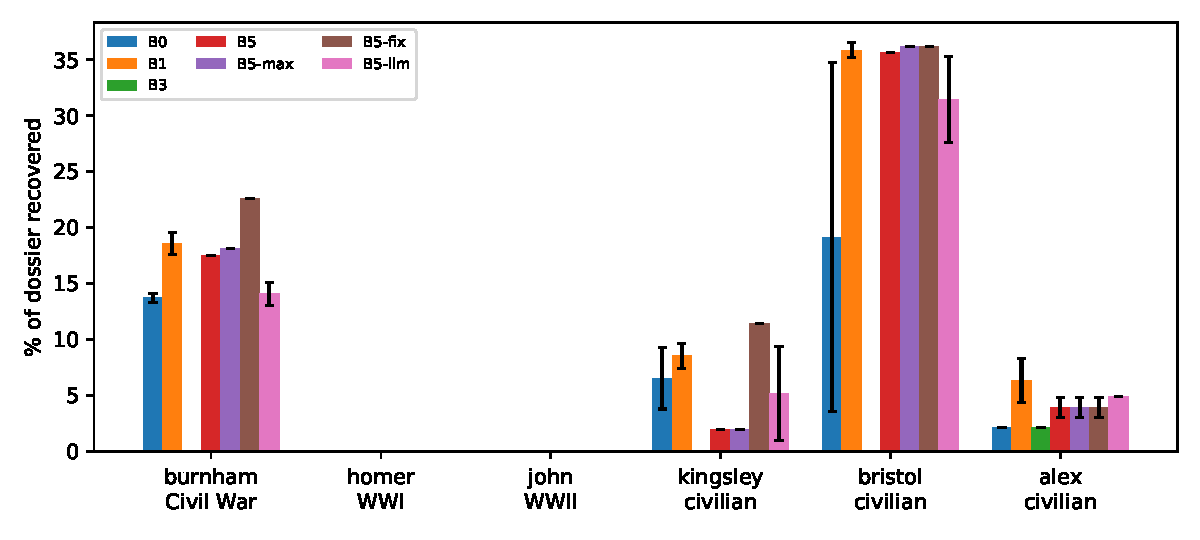
\includegraphics[width=0.92\textwidth]{figures/corpus-recall.pdf}}{\NM}
\caption{Share of each dossier recovered, per person and strategy, mean and sd over runs. Generated by \texttt{eval/corpus/report.py}.}
\label{fig:corpus}
\end{figure*}

\paragraph{The reachability ceiling is the larger finding.} Most dossier facts came from sources these tools cannot reach. Only \RESULT{corpus-reachn-homer} of Homer's facts and \RESULT{corpus-reachn-john} of John's have a source on archive.org, loc.gov or wikidata.org; their dossiers rest on obituaries in paywalled newspaper archives, military records behind logins, and family interviews. Every strategy scored zero on both. Scored on the reachable facts only (\cref{tab:reach}), B5 recovered \RESULT{corpus-reach-B5}, B1 \RESULT{corpus-reach-B1}, B0 \RESULT{corpus-reach-B0} and B5-fix \RESULT{corpus-reach-B5fix}. The ranking does not change, but the absolute numbers say that tool access, not question generation, sets the ceiling on this task.

\paragraph{Why CR underperformed (post hoc diagnosis).} We read the tool logs of every run (\cref{tab:diagnose}). Six causes stand out.
\begin{enumerate}
\item \emph{It stops early.} The preregistered B5 used \RESULT{diag-calls-B5} tool calls per run of its 100; its rule generator ran out of new questions. B1 used \RESULT{diag-calls-B1}.
\item \emph{It repeats itself.} \RESULT{diag-repeat-B5} of B5's calls, and \RESULT{diag-repeat-B5max} of B5-max's, were exact repeats of an earlier call in the same run, mostly the same search inside the same book asked again from different branches of the graph. ReAct repeated \RESULT{diag-repeat-B1}.
\item \emph{The checklist assumes a birthplace.} With only a name and a year, the checklist built empty queries (a title search for a town it did not have) and searched the full name with its middle name only; B3 scored zero for five of six people and \RESULT{diag-empty-B3} of its calls came back empty.
\item \emph{Name forms.} The rule generator parsed ``Homer Doble St.\ John'' with the surname ``John'' and never tried ``H.\ D.\ St.\ John'' or ``Homer D.\ St.\ John'', the forms the records use.
\item \emph{Namesakes.} Its searches pulled in the father and the son who share Burnham's name, and one passage about the father produced the wrong-parents link.
\item \emph{A model generator did not help here.} CR with a model writing its questions (B5-llm) recovered \RESULT{corpus-overall-B5llm}, below the rule generator, and the items it cited were less often about the subject (precision \RESULT{corpus-prec-B5llm}). On the record-level benchmark the same generator was the best CR variant (\cref{tab:ablate}), so the evidence on model-written questions is mixed.
\end{enumerate}
B5-fix repairs the second, fourth and part of the first cause (a ``St.''\ surname particle rule, name forms, de-duplication of planned calls, and continuing until the budget or the leads run out). It lifted CR from \RESULT{corpus-overall-B5} to \RESULT{corpus-overall-B5fix}, but it was tuned while looking at Burnham, so it is post hoc and its edge over B1 is not a test.

\begin{table*}[t]\centering\small
\begin{tabular}{@{}lcccccccc@{}}
\toprule
Strategy & Calls/run & Exact repeats & Empty results & Items returned & On target & IA full text & Inside a book & Newspapers \\
\midrule
B0 & 7.4 & 0.0\% & 50.2\% & 21 & 33.1\% & 2.1 & 0.0 & 2.2 \\
B1 & 22.4 & 0.6\% & 49.5\% & 466 & 22.7\% & 5.3 & 4.8 & 4.9 \\
B3 & 7.2 & 30.4\% & 75.6\% & 7 & 22.8\% & 0.0 & 0.0 & 1.2 \\
B5 & 17.0 & 41.4\% & 48.5\% & 537 & 42.2\% & 2.5 & 4.0 & 3.5 \\
B5-max & 41.8 & 52.7\% & 37.7\% & 1413 & 32.3\% & 2.8 & 24.1 & 6.3 \\
B5-fix & 46.4 & 11.1\% & 39.8\% & 1105 & 15.1\% & 3.8 & 23.0 & 10.4 \\
B5-llm & 42.3 & 26.3\% & 50.3\% & 121 & 49.4\% & 18.9 & 1.2 & 13.4 \\
\bottomrule
\end{tabular}
\caption{Tool-use profile per run on the corpus, from the tool-layer logs (\texttt{eval/corpus/diagnose.py}). Exact repeats: calls identical to an earlier call in the same run. On target: share of returned items that name the subject and carry no year outside his life. The last three columns are calls per run to each tool.}
\label{tab:diagnose}
\end{table*}


\paragraph{Scorer audit.} The scorer is automatic, so we audited it. A model judge at temperature 0 saw \RESULT{corpus-audit-n} sampled decisions, half credited and half not, with the exact text window the scorer matched. It agreed with the scorer on \RESULT{corpus-audit-agree} (Cohen's $\kappa=$\,\RESULT{corpus-audit-kappa}) and confirmed \RESULT{corpus-audit-prec} of credited facts. An AI research assistant then read every disagreement against the matched text (a second reading, not a human rating): \RESULT{corpus-hand-summary}. The first audit, on scorer version 1.0, found six bugs that inflated scores, among them an 1864 Homer D.\ St.\ John counting as the World War~I veteran, Burnham's father counting as Burnham, and loc.gov URLs that echo the agent's own query. We fixed them (scorer v1.1) and report v1.1 throughout; under v1.0 every overall score was higher or equal and the ranking was the same. Read the absolute numbers as upper bounds: about one credited fact in five is not supported by its evidence.

\paragraph{Leakage.} No call reached a blocked host (\cref{tab:leak}). The content guard dropped \RESULT{corpus-dropped-B1} items for B1, \RESULT{corpus-dropped-B5max} for B5-max, \RESULT{corpus-dropped-B5fix} for B5-fix and \RESULT{corpus-dropped-B5llm} for B5-llm; we read them, and every one was a page of a primary source that the dossiers quote at length (the 1884 Burnham genealogy and catalogue records of a book about Alex St.\ John), not a copy of the author's work. The guard is therefore conservative: it cost the strategies a little recall, evenly.

\begin{table}[t]\centering\small
\begin{tabular}{@{}lccc@{}}\toprule
Strategy & Runs & Host blocks & Overlap drops \\\midrule
B0 & 18 & \RESULT{corpus-blocked-B0} & \RESULT{corpus-dropped-B0} \\
B1 & 18 & \RESULT{corpus-blocked-B1} & \RESULT{corpus-dropped-B1} \\
B3 & 18 & \RESULT{corpus-blocked-B3} & \RESULT{corpus-dropped-B3} \\
B5 & 18 & \RESULT{corpus-blocked-B5} & \RESULT{corpus-dropped-B5} \\
B5-max & 18 & \RESULT{corpus-blocked-B5max} & \RESULT{corpus-dropped-B5max} \\
B5-fix & 18 & \RESULT{corpus-blocked-B5fix} & \RESULT{corpus-dropped-B5fix} \\
B5-llm & 18 & \RESULT{corpus-blocked-B5llm} & \RESULT{corpus-dropped-B5llm} \\\bottomrule
\end{tabular}
\caption{Leakage audit: tool calls blocked by the host rule and returned items dropped by the dossier 8-gram guard, all runs.}
\label{tab:leak}
\end{table}

\section{v0.2: a lane swarm with a search ledger}
\label{sec:swarm}

\paragraph{Why.} The v0.1 diagnosis (\cref{sec:corpus}) found that CR wasted calls on exact repeats, stopped before its budget, and that strategies used very different shares of the budget. v0.2 changes how calls are spent and adds a budget-matched comparison. The design is in \texttt{docs/v0.2-design.md}; the hypotheses, weights, comparators and decision rule were committed in \texttt{bench/PREREGISTRATION-v0.2.md} before any v0.2 live run.

\paragraph{Design.} An outline of research lanes (reference works, military service when the person was of age for a war, census, church, newspapers in three life phases, land, probate, immigration) is planned from the card alone, after STORM and Co-STORM~\cite{shao2024storm,jiang2024costorm}. Lanes run as parallel Temporal child workflows, four at a time~\cite{temporalpythonsdk}, following the parallel-subagent pattern of~\cite{anthropic2025multiagent} and guarding against the duplicated-work failure in~\cite{cemri2025mast}. Every call passes a run-wide search ledger in the orchestrator: exact and near repeats are refused before they cost anything, and a source may be revisited only with a new key (a name variant, adjacent pages, a gated relative's name, another collection, another date window, the next results page), once per value, with the reason logged. This is tabu search with aspiration criteria~\cite{glover1997tabu}, with name variants from record linkage~\cite{christen2012datamatching} and a foraging stop after three empty calls~\cite{pirolli1999foraging}. Within a lane, leads are picked by a value score plus a UCT bonus~\cite{kocsis2006uct,zhou2024lats}; a UCB1 allocator~\cite{auer2002ucb} splits calls across lanes; short rule-based lessons between rounds adjust expected yields~\cite{shinn2023reflexion}. A verification gate admits a citation only if the snippet prints the full name inside the life window. v0.2 adds the Internet Archive full-text search API~\cite{iafts}; B1 gets it too. B6 uses no model, so its model spend is zero.

\paragraph{Protocol.} Same six people, answer key, scorer rules, exclusion filter and $B=100$ as \cref{sec:corpus}. B1, B5 and B5-fix were rerun in the same batch, from the same commit (\RESULT{v02-commit}), with \RESULT{v02-runs} runs per person; v0.1 numbers are context only. Every run was also re-scored from its first $N$ logged calls, where $N$ is the median number of calls B1 used (\RESULT{v02-matchedN}), and at 10, 25, 50, 75 and 100 calls (\cref{fig:rvc}).

\IfFileExists{generated/v02-table.tex}{\begin{table*}[t]\centering\small
\resizebox{\textwidth}{!}{\begin{tabular}{@{}lcccccccccccc@{}}
\toprule
Strategy & Burnham & Homer & John & Kingsley & Bristol & Alex & Overall & Reachable & Precision & Calls & Repeats & Spend \\
\midrule
B6-swarm & 16.1$\pm$0.3 & 0.0$\pm$0.0 & 0.7$\pm$0.6 & 11.6$\pm$0.0 & 29.9$\pm$0.0 & 10.9$\pm$0.0 & 11.5\% & 22.7\% & 76.3\% & 94.4 & 0.4\% & \$0.00 \\
B6-no-ledger & 15.9$\pm$0.0 & 0.0$\pm$0.0 & 0.7$\pm$0.6 & 12.7$\pm$0.0 & 29.9$\pm$0.0 & 11.4$\pm$0.0 & 11.8\% & 23.1\% & 80.2\% & 94.4 & 13.5\% & \$0.00 \\
B6-no-parallel & 16.1$\pm$0.3 & 0.0$\pm$0.0 & 1.0$\pm$0.0 & 11.6$\pm$0.0 & 29.9$\pm$0.0 & 10.9$\pm$0.0 & 11.6\% & 22.7\% & 76.0\% & 94.4 & 0.3\% & \$0.00 \\
B5-fix & 22.6$\pm$0.0 & 0.0$\pm$0.0 & 0.0$\pm$0.0 & 11.4$\pm$0.0 & 36.2$\pm$0.0 & 4.4$\pm$0.9 & 12.4\% & 24.6\% & 67.3\% & 52.2 & 7.0\% & \$0.00 \\
B5 & 17.5$\pm$0.0 & 0.0$\pm$0.0 & 0.0$\pm$0.0 & 1.9$\pm$0.0 & 35.6$\pm$0.0 & 4.4$\pm$0.9 & 9.9\% & 19.7\% & 66.8\% & 22.7 & 37.5\% & \$0.00 \\
B1 & 18.5$\pm$1.1 & 0.0$\pm$0.0 & 0.0$\pm$0.0 & 8.0$\pm$1.7 & 35.6$\pm$0.6 & 12.0$\pm$1.5 & 12.4\% & 24.1\% & 55.8\% & 22.2 & 1.1\% & \$0.47 \\
\bottomrule
\end{tabular}}
\caption{v0.2 corpus replication at $B=100$ (answer key v1, scorer v1.1), percent of each dossier recovered, mean$\pm$sd over runs. All strategies were rerun in the same batch from the same commit with the same tools (B1 also has \texttt{ia\_fts}). Repeats: share of logged calls that repeat an earlier successful call with the same arguments (retries of failed calls excluded). Spend: model dollars over all runs. Generated by \texttt{eval/fill\_v02.py}.}
\label{tab:v02}
\end{table*}
}{}

\paragraph{Results.} B6-swarm recovered \RESULT{v02-overall-B6-swarm} of the dossiers on average, against \RESULT{v02-overall-B1} for B1 and \RESULT{v02-overall-B5-fix} for B5-fix (B5: \RESULT{v02-overall-B5}). Against B1 the mean per-person difference was \RESULT{v02-B6-swarm-vs-B1-diff} points (\RESULT{v02-B6-swarm-vs-B1-wl}, exact sign-flip $p=$\,\RESULT{v02-B6-swarm-vs-B1-p}, Holm $p=$\,\RESULT{v02-B6-swarm-vs-B1-holm}); against B5-fix it was \RESULT{v02-B6-swarm-vs-B5-fix-diff} points (\RESULT{v02-B6-swarm-vs-B5-fix-wl}, $p=$\,\RESULT{v02-B6-swarm-vs-B5-fix-p}). Precision was \RESULT{v02-prec-B6-swarm} for B6-swarm, \RESULT{v02-prec-B5-fix} for B5-fix and \RESULT{v02-prec-B1} for B1. B6-swarm's exact-repeat rate was \RESULT{v02-waste-repeat} and it used \RESULT{v02-waste-used} of $B$. The ablations recovered \RESULT{v02-overall-B6-no-ledger} without the ledger and \RESULT{v02-overall-B6-no-parallel} with one worker. At the matched call count, B6-swarm recovered \RESULT{v02-matched-overall-B6-swarm} against \RESULT{v02-matched-overall-B1} for B1. Model spend for the whole batch was \RESULT{v02-usd-total}, all of it B1's (\RESULT{v02-tokens-B1} tokens); B5 and B6 used \RESULT{v02-tokens-B6-swarm} model tokens.

\IfFileExists{generated/v02-h6-table.tex}{\begin{table}[t]\centering\small
\begin{tabular}{@{}p{0.17\linewidth}p{0.5\linewidth}l@{}}
\toprule
Hypothesis & Preregistered test & Verdict \\
\midrule
H6 & B6-swarm beats B1 and B5-fix on overall recall & NOT SUPPORTED \\
H6-prec & precision within 3 points of B5-fix and above B1 & SUPPORTED \\
H6-waste & exact-repeat rate below 2\% and at least 80\% of B used & SUPPORTED \\
H6-ablation & B6-swarm beats B6-no-ledger and B6-no-parallel & NOT SUPPORTED \\
H6-budget & B6-swarm beats B1 at the matched call count & NOT SUPPORTED \\
\bottomrule
\end{tabular}
\caption{Preregistered v0.2 hypotheses (\texttt{bench/PREREGISTRATION-v0.2.md}) and verdicts under the preregistered decision rule, computed by \texttt{eval/corpus/h6.py}. With six people no difference can be statistically significant.}
\label{tab:h6}
\end{table}
}{}

\paragraph{Verdicts.} Under the preregistered rule (\cref{tab:h6}): H6 \RESULT{v02-H6}; H6-prec \RESULT{v02-H6-prec}; H6-waste \RESULT{v02-H6-waste}; H6-ablation \RESULT{v02-H6-ablation}; H6-budget \RESULT{v02-H6-budget}. \textbf{Six people are far too few for statistical significance}: only four have reachable facts, so the smallest attainable two-sided $p$ on those is 0.125, and the permutation and Holm $p$ values above are reported for completeness, not as evidence.

\paragraph{Failed runs.} \RESULT{v02-failed} of the \RESULT{v02-nruns} runs ended with a Temporal client timeout (\texttt{RPCError: Timeout expired}) during an infrastructure hiccup on the benchmark machine: \RESULT{v02-failed-list}. They are kept and scored as run, as the harness logs every run and drops none: each logged some calls before the timeout but never returned a report, so it scores zero recall and counts zero charged calls. This lowers the swarm's mean share of $B$ used and touches John and Homer, whose dossiers are almost unreachable. As a \emph{post hoc} sensitivity check we reran only those four runs from the same commit (\RESULT{v02s-failed} failed runs remain; aggregates in \texttt{benchmark/results/v1/v0.2-rerun4-posthoc}): B6-swarm then recovered \RESULT{v02s-overall-B6-swarm} (B1 \RESULT{v02s-overall-B1}, B5-fix \RESULT{v02s-overall-B5-fix}), and the verdicts were H6 \RESULT{v02s-H6}, H6-prec \RESULT{v02s-H6-prec}, H6-waste \RESULT{v02s-H6-waste}, H6-ablation \RESULT{v02s-H6-ablation}, H6-budget \RESULT{v02s-H6-budget}. The preregistered verdicts are the ones above.

\paragraph{Reading the result.} The ledger did what it was built to do: B6-swarm almost never repeated a call (\RESULT{v02-repeat-B6-swarm}, against \RESULT{v02-repeat-B5} for B5 and \RESULT{v02-repeat-B6-no-ledger} for the same swarm without the ledger) and spent nearly the whole budget, where B1 stopped after about \RESULT{v02-calls-B1} calls. It did not turn those calls into more recovered facts. Empty calls were common (\RESULT{v02-empty-B6-swarm} of B6-swarm's calls), and the curve (\cref{fig:rvc}) shows the swarm behind B1 and B5-fix at matched budgets and still below them at 100 calls. The ablations were within a point of the full swarm, so neither the ledger nor parallelism changed recall on this task; the reachability ceiling of \cref{sec:corpus} still binds. These readings are descriptive; six people cannot separate the strategies.

\begin{figure}[t]\centering
\RESULTFIG{recall-vs-calls}{overall recall after 10, 25, 50, 75 and 100 logged calls per strategy}
\caption{Recall against tool calls: every run re-scored from its first $N$ logged calls (\texttt{eval/corpus/report.py --truncate-calls}). Drawn by \texttt{eval/plots.py}.}
\label{fig:rvc}
\end{figure}

\IfFileExists{generated/v02-diagnose-table.tex}{\begin{table}[t]\centering\small
\begin{tabular}{@{}lcccc@{}}
\toprule
Strategy & Repeats & Repeats incl.\ retries & Empty & Wikidata 429s \\
\midrule
B6-swarm & 0.4\% & 1.6\% & 49.7\% & 0 \\
B6-no-ledger & 13.5\% & 19.4\% & 47.0\% & 0 \\
B6-no-parallel & 0.3\% & 1.4\% & 49.7\% & 0 \\
B5-fix & 7.0\% & 8.3\% & 38.2\% & 0 \\
B5 & 37.5\% & 41.0\% & 47.8\% & 0 \\
B1 & 1.1\% & 1.1\% & 38.0\% & 0 \\
\bottomrule
\end{tabular}
\caption{v0.2 tool-use profile from the tool logs (\texttt{eval/corpus/diagnose.py}).}
\label{tab:v02diag}
\end{table}
}{}

\paragraph{Post hoc feature: search graph and cache.} \emph{Added after the preregistration and not part of any benchmark condition.} Each swarm run can export a persistent search graph built from its ledger (\texttt{cr/search\_graph.py}): nodes for the person, relatives used as keys, places, queries, sources and records; edges with provenance (which query found which record, which record supports which ``Possible'' finding, with a capped snippet, and which revisit was allowed for which reason). A later run can load earlier graphs as a cache and skip queries already done, at no budget cost. The cache is off for every benchmark condition and the v0.2 batch ran from a commit without it, so none of the numbers above depend on it. \Cref{fig:graph} shows the graph exported, after the batch, for one preregistered B6-swarm run on Burnham.

\begin{figure*}[t]\centering
\IfFileExists{figures/search-graph-burnham.pdf}{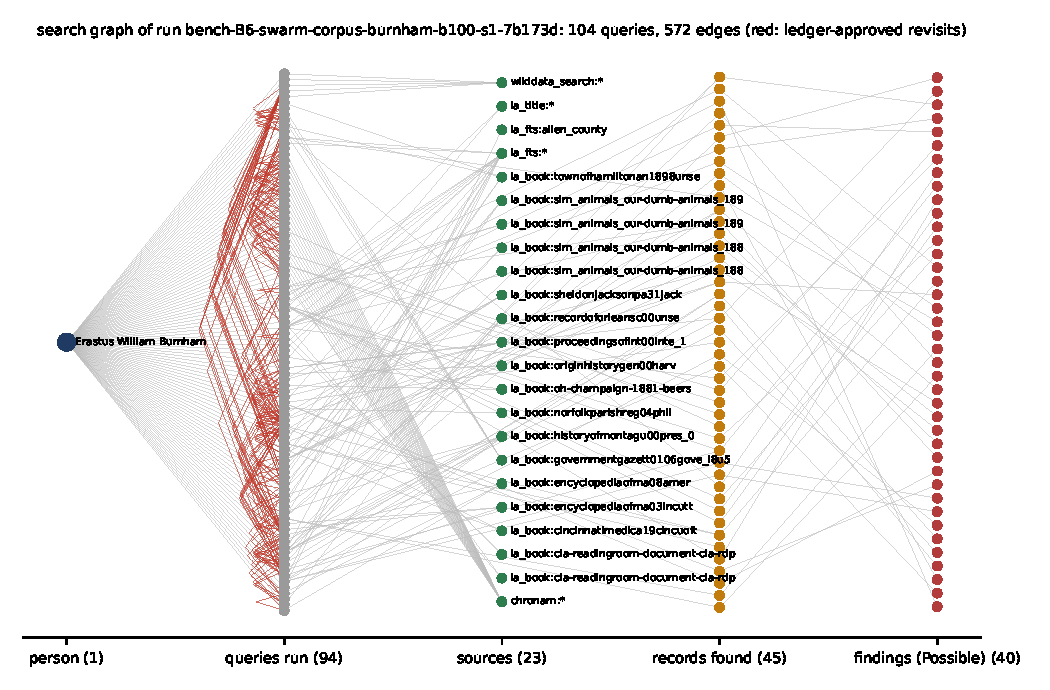
\includegraphics[width=0.9\textwidth]{figures/search-graph-burnham.pdf}}{\NM}
\caption{Search graph of one B6-swarm run (Burnham, seed 1), exported from its ledger by \texttt{scripts/export\_graph.py} and drawn by \texttt{scripts/plot\_graph.py}: the person, the queries the run executed, the sources they searched, the records they returned and the findings (all ``Possible'') those records support. Red arcs are ledger-approved revisits of an earlier query. Post hoc figure; no snippet text is drawn.}
\label{fig:graph}
\end{figure*}

\section{Results}
\label{sec:results}

\subsection{Main comparison (H1, H4)}
\Cref{tab:main} reports $B=100$ on \RESULT{n-subjects-test} test subjects.
\begin{table*}[t]
\centering\small
\begin{tabular}{@{}lccccc@{}}
\toprule
Agent at $B=100$ & Recall@100 [95\% CI] & T1 recall & T3 identification & Claim precision & Wrong person \\
\midrule
B0 single pass & \RESULT{H1-recall-B0-B100} & \RESULT{H1b-T1-B0} & \RESULT{H1b-T3-B0} & \RESULT{H4-prec-B0} & \RESULT{wp-B0} \\
B1 ReAct & \RESULT{H1-recall-B1-B100} & \RESULT{H1b-T1-B1} & \RESULT{H1b-T3-B1} & \RESULT{H4-prec-B1} & \RESULT{wp-B1} \\
B3 checklist only & \RESULT{H1-recall-B3-B100} & \RESULT{H1b-T1-B3} & \RESULT{H1b-T3-B3} & \RESULT{H4-prec-B3} & \RESULT{wp-B3} \\
B5 full system & \RESULT{H1-recall-B5-B100} & \RESULT{H1b-T1-B5} & \RESULT{H1b-T3-B5} & \RESULT{H4-prec-B5} & \RESULT{wp-B5} \\
\bottomrule
\end{tabular}
\caption{Main results at $B=100$ on the \bench test split, 3 seeds where a model is used; the subject count is in the text. Wilcoxon with Holm correction, bootstrap CIs.}
\label{tab:main}
\end{table*}

\begin{figure*}[t]
\centering
\newcommand{\cell}[4]{\begin{minipage}[t]{0.24\textwidth}\centering\resizebox{\linewidth}{!}{\RESULTFIG{#1}{#2}}\captionof{figure}{#3}\label{#4}\end{minipage}}
\cell{fig5-recall-budget}{Recall@$B$, B0 to B5, $B\in\{25,50,100\}$, 95\% CI bands.}{Recall versus budget.}{fig:budget}\hfill
\cell{fig6-recall-tier}{Recall by tier T0 to T3 per agent, $B=100$.}{Recall by darkness tier.}{fig:tier}\hfill
\cell{fig7-completion-faults}{Completion vs.\ failure rate $p$, with and without kills, B5 vs.\ B4.}{Completion under faults.}{fig:faults}\hfill
\cell{fig8-depth-to-hit}{Depth of the node that first found each hidden record (B5).}{Lead-chain depth to hit.}{fig:depth}
\end{figure*}

\subsection{Durability (H2), memory (H3) and nudging (H5)}

Under kills and $p=0.3$, B5 completed \RESULT{H2-complete-B5} of runs and B4 \RESULT{H2-complete-B4} (McNemar $p=$\,\RESULT{H2-mcnemar-p}); the duplicate-work ratio was \RESULT{H2-dup-B5} for B5 and \RESULT{H2-dup-B4} for B4. With memory on, cost to reach the first run's recall fell from \RESULT{H3-cost-off} to \RESULT{H3-cost-on} tool calls. Nudge coverage was \RESULT{H5-coverage-B5} for B5 and \RESULT{H5-coverage-B3} for B3 (coder kappa \RESULT{H5-kappa}). \Cref{tab:nudge,tab:cost,tab:ablate} are in the appendix.

\subsection{Pilot: what exists today}
\label{sec:pilot}
These are from local runs on 26 November 2026 on the Temporal dev server, computed by \texttt{eval/pilot\_stats.py} from the reference system's store and from its durability log. They are a pilot on 2 subjects, not a benchmark.
\begin{itemize}
\item \textbf{Runs.} 9 runs: 2 blocked by the living-person gate before any lookup (a test person born 1950), 6 approved through the API, 1 left awaiting approval. 7 runs built graphs: 5 for Erastus W.\ Burnham on the Civil War circuit and 2 for Mary Devine (1830 to 1911) on the crossing circuit, 132 question nodes in all (14, 31, 20, 16, 25, 12 and 14).
\item \textbf{Memory.} Every run after the first for a subject re-asked the earlier runs' top-level questions first (3 per run, ids \textit{r1} to \textit{r3}) and deduplicated new ideas against them.
\item \textbf{Outreach.} 6 drafted requests (the National Archives; the Connecticut State Library, State Archives; and four to a town or county clerk in Glasgow). 2 were approved and written to a local folder; none was sent.
\item \textbf{Durability.} The worker was killed with SIGKILL 5 times during runs. While it was down, Temporal held the runs with 74, 128, 87, 194 and 158 history events and lookups pending. After each restart the run continued from the same nodes. In the two histories checked (303 and 209 events), no activity was scheduled again after it had completed; in-flight lookups were retried after their 90\,s start-to-close timeout. Simulated flaky archives produced visible ``attempt 1 failed (simulated 503), retried by Temporal'' entries, up to 6 attempts on one node.
\item \textbf{A careful single pass misses most records.} The production system's single-pass search, measured on 2 November 2026 on two golden cases, had recall of 41.7\% (10 of 24) and 30.4\% (7 of 23), with precision 100\% and no wrong-person records. That is a different system and subject set, so it motivates the problem and is not a \bench baseline.
\end{itemize}

\subsection{Case studies}
\label{sec:cases}
\paragraph{Erastus W.\ Burnham, Civil War circuit.} The 12th Connecticut chain is in \cref{sec:worked}. Other live leads: ``Erastus Williams Burnham'' in four full-text book hits, and a book giving ``born April 28, 1834'', which matches the fixture. Fixtures list soldier entries for both the 1st Connecticut Heavy Artillery and the 12th Connecticut Infantry, an identity question left open.

\label{sec:wrongparents}
\paragraph{Error analysis: two wrong-parents leads.} In an early run the generator asked ``Who were his parents, Amos and Martha (Billings) Burnham?''\ from a line that actually read ``Lois E.\ Burnham, daughter of Amos and Martha (Billings)'', a different person. The fix required the subject's own given name just before ``son of''. A later run then produced ``Phineas and Abigail (Huntley)'' from a line that does name ``(VI) Erastus W.\ Burnham, son of Phineas and Abigail (Huntley) Burnham''. Its follow-up search for ``Phineas Burnham'' returned full-string matches about other people (a comic book, a 1958 periodical, an alumni magazine). The fix was not enough. When the evidence layer was added, it extracted every lead from the same passage and compared lead dates with documented ones: the passage continues ``was born April 15, 1810, and died October 20, 1854''. The documented record has 1834 to 1921. The report now names two conflicts (birth and death) and pulls the parents lead into both, with the note that the passage may describe a different man of the same name. Another book names an ``Erastus Williams Burnham, (son of Erastus W.'', which is consistent with an older Erastus, but that reading is itself a lead. This case motivates four design choices: grounding each question in a quoted finding, ``Are you sure?''\ nodes, the wrong-person metric, and treating name-string matches as leads that a conflict check can overturn.

\paragraph{Mary Devine and the gate.} The crossing circuit has no keyless source for passenger lists or naturalisation, so the loop drafted requests to a town or county clerk in Glasgow (T3 identification, ask first). A test person born in 1950 was blocked before any lookup.

\paragraph{Corpus cases.} On the corpus benchmark (\cref{sec:corpus}), Bristol, whose dossier is mostly reachable, is where the preregistered CR came closest to ReAct; Homer and John, whose dossiers are almost entirely unreachable with these tools, are where every strategy scored zero; Burnham is where the namesake father produced CR's false family links.

\section{Discussion: what we learned}
\label{sec:discussion}

\paragraph{Curiosity is the product.} The checklist alone answers the questions someone already thought to ask. The finds that mattered in the pilot came from questions the checklist did not contain: which books cover this regiment, does this book name him and on which page, who are the people this line calls his parents. Whether that holds at scale is H1, and on this benchmark it did not: a ReAct agent with the same tools and budget found more, and the rule generator stopped before its budget ran out (\cref{sec:corpus}). What CR kept was precision: the items it cited were more often about the right person.

\paragraph{The record of what was checked is what makes it trustworthy.} A run leaves its question graph, the finding behind every question, every retry and every human decision. That turns ``did the agent check the synagogues?''\ from a question about a black box into a lookup.

\paragraph{Leads must stay leads, and a second look must be able to overturn them.} The wrong-parents case (\cref{sec:wrongparents}) shows two things. A narrow rule fixed the first error and still let the second through. What caught the second was not a better pattern but keeping the whole quoted passage and checking it against documented facts. So we keep stubs labelled, keep quotes verbatim, and never let a name match decide a date or a family link.

\paragraph{Where durability did not matter.} For a 10-minute run with a healthy network, durable execution adds a server, a worker and determinism rules to the code, and buys little. It matters when the work is long (timers in days, replies in weeks), when sources are flaky, when a person must approve or redirect mid-run, and when someone later needs to know exactly what happened. H2 measures how much; we expect the gap to grow with run length. \RESULT{H2-discussion-gap}

\section{How this helps break out}
\label{sec:breakout}
A ``brick wall'' in genealogy is an ancestor whose parents are unknown; CR is meant to keep generating grounded questions at exactly that point, where a person would otherwise stop.

\section{Next steps}
\label{sec:future}
First, reach: the corpus benchmark shows that tool access, not question generation, capped every strategy, so keyed newspaper, military and vital-record sources under the user's own credentials come before any change to the generator. Then: fix the rule generator's early stop and repeated calls in the preregistered configuration and test B5-fix on held-out dossiers; add continue-as-new and per-subtree child workflows for week-long runs; share question memory across families for the same unit, ship or town; real outreach with per-message consent and follow-ups at 21 and 60 days; handwriting recognition over family boxes; a larger, multi-country \bench.

\section{Limitations and ethics}
\label{sec:limits}

\paragraph{Limitations.}
\begin{itemize}
\item The preregistered configuration uses the rule-based generator (templates in the appendix). The grounded model generator was measured only as an ablation (B5-llm), with mixed results: best CR variant on the record-level benchmark, below the rule generator on the corpus.
\item Corpus scores are automatic. A model audit and a second, item-by-item reading of every disagreement by an AI assistant put the scorer's precision near four in five credited facts, so absolute scores are upper bounds; the scorer was revised once (v1.0 to v1.1) after its first audit, uniformly for every strategy.
\item The corpus benchmark has six people, all from one family's research, and no held-out dossier: B5-fix was repaired while looking at Burnham. Its edge over ReAct is not a test.
\item The rule generator is deterministic, so its three runs per person differ only through live sources; their sd understates real variability.
\item In the pilot, most record-level facts come from curated evaluation fixtures, labelled stub. Live sources add leads, not facts. Every benchmark run switches the fixtures off.
\item A ``strong'' name match means the full name string appears in OCR text, not that it is the same person. In a comma-separated roster the name order must be read from the page.
\item Chronicling America queries are slow (about 30\,s); Internet Archive lending books refuse inside-book search (HTTP 403); catalogue title search returns books that share only a surname or a regiment number. From some cloud addresses Wikidata answers every call with HTTP 429.
\item No continue-as-new yet; time-skipping tests simulate days, not real archives.
\item Small $n$. The author built the system and much of the ground truth; independent raters and a sealed holdout are the mitigation. The benchmark skews toward the United States and New England and English-language records. Tiers are assigned by a host rule until a person confirms them.
\end{itemize}

\paragraph{Deviations from the preregistration.} (1) B0, B1 and the model generator used one xAI model (\texttt{grok-4.20-0309-non-reasoning}) instead of the preregistered provider. (2) B5-max (wider limits), B5-fix (repaired rules) and B5-llm on the corpus are post hoc and labelled so. (3) H2 ran as a pilot: four subjects, capped seeds and failure rates. (4) Scoring is automatic candidate matching; claim precision and the wrong-person rate need two human raters and are not measured (\NM). (5) The record-level H1 runs predate the exclusion filter; a retrospective check of every cited item, lead and final answer found no blocked host and no copied dossier text. (6) The corpus-replication benchmark, its exclusion filter and its scorer were designed after the preregistration. (7) Five corpus runs that failed on Temporal client timeouts were rerun with the same seeds; the failed attempts are kept in the run directory. (8) H1 ran at $B\in\{25,50,100\}$, not 200, with one seed at 25 and 50; B3 ran at 25 and 100 only. Two B1 runs (one at $B=25$, one at $B=50$) ended on a model API read timeout and are excluded, so those cells have 38 subjects.

\paragraph{Ethics.}
\begin{itemize}
\item \emph{Living people.} No living person is a benchmark subject, figure, example or case study. The gate runs in workflow code before any lookup, and an unknown date means living. Living relatives named in a deceased person's records (for example an interviewee) are redacted in anything released; six family dossiers whose subjects are deceased are released as atomic facts with citations and identifiers only, never book or page contents; facts about living relatives stay in a private set that is scored locally and published only as aggregates.
\item \emph{Family privacy.} Private items (interviews, photo boxes) are released only as counts and tiers; the author's transcripts are used with his consent.
\item \emph{Archive terms and consent.} No scraping where terms forbid it (Find a Grave is links only), no captcha or paywall bypass, polite rate limits, a contact address in the user agent. Nothing is sent: real outreach needs approval per message, and the benchmark's archives are simulated.
\item \emph{Sensitive records.} Religious, adoption, institutional, enslavement and Indigenous records carry community rules; the system defers to them.
\item \emph{Misidentification harm.} A wrong-person attribution can rewrite a family's story, so leads are labelled and conflicts named.
\end{itemize}


\bibliographystyle{plainnat}
\bibliography{refs}

\appendix
\section{Further results tables}
\begin{table}[t]
\centering\small
\resizebox{\columnwidth}{!}{\begin{tabular}{@{}lcc@{}}
\toprule
Ablation (B5, $B=100$, dev split) & Recall@100 & Wrong-person rate \\
\midrule
Full system & \RESULT{abl-full} & \RESULT{abl-full-wp} \\
Breadth $b=1$ / 3 / 5 / 8 & \RESULT{abl-breadth} & \RESULT{abl-breadth-wp} \\
Depth $d_{\max}=1$ / 2 / 3 / 4 & \RESULT{abl-depth} & \RESULT{abl-depth-wp} \\
Node budget $N=10$ / 30 / 50 / 80 & \RESULT{abl-nodes} & \RESULT{abl-nodes-wp} \\
Memory off & \RESULT{abl-nomem} & \RESULT{abl-nomem-wp} \\
Generator: grounded model / hybrid & \RESULT{abl-gen} & \RESULT{abl-gen-wp} \\
Circuits off & \RESULT{abl-nocircuits} & \RESULT{abl-nocircuits-wp} \\
``Are you sure?'' nodes off & \RESULT{abl-noverify} & \RESULT{abl-noverify-wp} \\
Dedupe off & \RESULT{abl-nodedupe} & \RESULT{abl-nodedupe-wp} \\
\bottomrule
\end{tabular}}
\caption{Ablations (Table 4). Harness agent names: \texttt{B5}, \texttt{B5-nomem}, \texttt{B5-llm}, \texttt{B5-hybrid}, \texttt{B5-nocircuits}, \texttt{B5-noverify}, \texttt{B5-nodedupe}.}
\label{tab:ablate}
\end{table}

\begin{table}[t]
\centering\small
\resizebox{\columnwidth}{!}{\begin{tabular}{@{}lccc@{}}
\toprule
Nudge type (coded from the transcripts) & Instances & Generated by B3 & Generated by B5 \\
\midrule
Deepen (``go deeper'') & \RESULT{n-deepen} & \RESULT{c3-deepen} & \RESULT{c5-deepen} \\
Verify (``are you sure?'') & \RESULT{n-verify} & \RESULT{c3-verify} & \RESULT{c5-verify} \\
Broaden to a named source type & \RESULT{n-broaden} & \RESULT{c3-broaden} & \RESULT{c5-broaden} \\
New source idea & \RESULT{n-new} & \RESULT{c3-new} & \RESULT{c5-new} \\
Follow up on an archive & \RESULT{n-follow} & \RESULT{c3-follow} & \RESULT{c5-follow} \\
Ingest or save & \RESULT{n-ingest} & \RESULT{c3-ingest} & \RESULT{c5-ingest} \\
Keep going & \RESULT{n-keep} & \RESULT{c3-keep} & \RESULT{c5-keep} \\
\midrule
Coder agreement (kappa) & \multicolumn{3}{c}{\RESULT{nudge-kappa}} \\
\bottomrule
\end{tabular}}
\caption{Nudge taxonomy and coverage (Table 5). Two coders; Cohen's kappa is in the last row.}
\label{tab:nudge}
\end{table}

\begin{table}[t]
\centering\small
\resizebox{\columnwidth}{!}{\begin{tabular}{@{}lcccc@{}}
\toprule
Agent & Tool calls & Tokens & Dollars & Wall-clock \\
\midrule
B0 & \RESULT{cost-B0-calls} & \RESULT{cost-B0-tok} & \RESULT{cost-B0-usd} & \RESULT{cost-B0-time} \\
B1 & \RESULT{cost-B1-calls} & \RESULT{cost-B1-tok} & \RESULT{cost-B1-usd} & \RESULT{cost-B1-time} \\
B3 & \RESULT{cost-B3-calls} & 0 & 0 & \RESULT{cost-B3-time} \\
B5 & \RESULT{cost-B5-calls} & 0 (rules) & 0 (rules) & \RESULT{cost-B5-time} \\
\bottomrule
\end{tabular}}
\caption{Cost per verified record (Table 6). The rule-based generator calls no model; keyless sources cost nothing but time.}
\label{tab:cost}
\end{table}

\section{Schemas, circuits and templates}
\paragraph{Typed schemas.} Every value that crosses Temporal is a Pydantic model: \texttt{Person}; \texttt{ResearchRequest} (with the CR switches: generator, memory, circuits, verification nodes, dedupe, fixtures, budgets); \texttt{Finding}, \texttt{Claim}, \texttt{Citation}; \texttt{Question} (the graph node), \texttt{Plan}; \texttt{Lead} and \texttt{Conflict}; \texttt{OutreachDraft} and \texttt{ArchiveReply}; \texttt{Progress} (the query); and \texttt{StudioReport}, whose sentences each carry claim ids.

\paragraph{Circuits.} YAML files: \texttt{civil\_war\_veteran} (unit and service dates, burial, pension file, census households, birth, marriage, parents, work before and after the war), \texttt{the\_crossing} (birthplace abroad, passage and arrival, naturalisation, marriage, where they settled, photographs, death and burial, parents) and \texttt{vital\_records} (birth, marriage, work and schooling, census and addresses, children, death and burial, parents), over 20 steps: 7 live, 13 stub with their reasons.

\paragraph{Lead templates (rule generator).} name to books; unit to books and newspapers; ship to voyages and newspapers; snippet ``son of A and B'' to parents, and to grandparents for a parent's line; snippet collection to a letter; marriage to the church; school to registers; congregation to its records; place to the church; death year to an obituary; book hit to search inside the book; Wikidata match to relatives; every node: ``Are you sure?''\ and ``Where else might this be?''; checklist gap to ``Still nothing on $X$''.

\paragraph{Grounded model generator.} The model gets the subject, the spark texts with ids, the question chain above the node, every question asked, the checklist gaps and the runnable handlers, and must return JSON questions with a spark id, a quote of 3 to 12 words from that spark, and a plan. Code rejects any question whose spark id is unknown, whose quote is not in the spark, or whose plan cannot run. The prompt is in \texttt{cr/generators/llm.py}.

\section{Reproducibility checklist}
\begin{itemize}
\item Code, the public part of the data, configurations and seeds are released; every results line records the commit hash.
\item Versions: Python 3.13, Temporal CLI 1.10.1 (server 1.32.2), Temporal Python SDK 1.37.0. Model names and dates: \RESULT{model-versions}.
\item Budgets, stopping rules and settings are in each results line; the preregistration is local commit \texttt{c6b7a6b} (26 November 2026), to be replaced by the public repository's first commit of \texttt{bench/PREREGISTRATION.md}.
\item Subjects, ground truth and the holdout procedure are in the datasheet; the living-person filter is applied and logged.
\item Source access dates are logged per run; archives change.
\item Fault settings and seeds are written into every fault-run line.
\item Adjudication guide, rater qualifications and kappa: \texttt{eval/adjudicate/}; kappa \RESULT{rater-kappa}.
\item Compute and dollars for all experiments: \RESULT{total-cost}.
\end{itemize}

\section{Placeholders still to fill}
This draft contains \arabic{tbdcount} placeholders. Each is filled from a logged results file, or the paper says it was not measured.
\printtbd

\end{document}
